
%% bare_conf.tex
%% V1.3
%% 2007/01/11
%% by Michael Shell
%% See:
%% http://www.michaelshell.org/
%% for current contact information.
%%
%% This is a skeleton file demonstrating the use of IEEEtran.cls
%% (requires IEEEtran.cls version 1.7 or later) with an IEEE conference paper.
%%
%% Support sites:
%% http://www.michaelshell.org/tex/ieeetran/
%% http://www.ctan.org/tex-archive/macros/latex/contrib/IEEEtran/
%% and
%% http://www.ieee.org/

%%*************************************************************************
%% Legal Notice:
%% This code is offered as-is without any warranty either expressed or
%% implied; without even the implied warranty of MERCHANTABILITY or
%% FITNESS FOR A PARTICULAR PURPOSE! 
%% User assumes all risk.
%% In no event shall IEEE or any contributor to this code be liable for
%% any damages or losses, including, but not limited to, incidental,
%% consequential, or any other damages, resulting from the use or misuse
%% of any information contained here.
%%
%% All comments are the opinions of their respective authors and are not
%% necessarily endorsed by the IEEE.
%%
%% This work is distributed under the LaTeX Project Public License (LPPL)
%% ( http://www.latex-project.org/ ) version 1.3, and may be freely used,
%% distributed and modified. A copy of the LPPL, version 1.3, is included
%% in the base LaTeX documentation of all distributions of LaTeX released
%% 2003/12/01 or later.
%% Retain all contribution notices and credits.
%% ** Modified files should be clearly indicated as such, including  **
%% ** renaming them and changing author support contact information. **
%%
%% File list of work: IEEEtran.cls, IEEEtran_HOWTO.pdf, bare_adv.tex,
%%                    bare_conf.tex, bare_jrnl.tex, bare_jrnl_compsoc.tex
%%*************************************************************************

% *** Authors should verify (and, if needed, correct) their LaTeX system  ***
% *** with the testflow diagnostic prior to trusting their LaTeX platform ***
% *** with production work. IEEE's font choices can trigger bugs that do  ***
% *** not appear when using other class files.                            ***
% The testflow support page is at:
% http://www.michaelshell.org/tex/testflow/



% Note that the a4paper option is mainly intended so that authors in
% countries using A4 can easily print to A4 and see how their papers will
% look in print - the typesetting of the document will not typically be
% affected with changes in paper size (but the bottom and side margins will).
% Use the testflow package mentioned above to verify correct handling of
% both paper sizes by the user's LaTeX system.
%
% Also note that the "draftcls" or "draftclsnofoot", not "draft", option
% should be used if it is desired that the figures are to be displayed in
% draft mode.
%
\documentclass[conference]{ieee/IEEEtran}
% Add the compsoc option for Computer Society conferences.
%
% If IEEEtran.cls has not been installed into the LaTeX system files,
% manually specify the path to it like:
% \documentclass[conference]{../sty/IEEEtran}

 



% Some very useful LaTeX packages include:
% (uncomment the ones you want to load)


% *** MISC UTILITY PACKAGES ***
%
%\usepackage{ifpdf}
% Heiko Oberdiek's ifpdf.sty is very useful if you need conditional
% compilation based on whether the output is pdf or dvi.
% usage:
% \ifpdf
%   % pdf code
% \else
%   % dvi code
% \fi
% The latest version of ifpdf.sty can be obtained from:
% http://www.ctan.org/tex-archive/macros/latex/contrib/oberdiek/
% Also, note that IEEEtran.cls V1.7 and later provides a builtin
% \ifCLASSINFOpdf conditional that works the same way.
% When switching from latex to pdflatex and vice-versa, the compiler may
% have to be run twice to clear warning/error messages.






% *** CITATION PACKAGES ***
%
\usepackage{cite}
% cite.sty was written by Donald Arseneau
% V1.6 and later of IEEEtran pre-defines the format of the cite.sty package
% \cite{} output to follow that of IEEE. Loading the cite package will
% result in citation numbers being automatically sorted and properly
% "compressed/ranged". e.g., [1], [9], [2], [7], [5], [6] without using
% cite.sty will become [1], [2], [5]--[7], [9] using cite.sty. cite.sty's
% \cite will automatically add leading space, if needed. Use cite.sty's
% noadjust option (cite.sty V3.8 and later) if you want to turn this off.
% cite.sty is already installed on most LaTeX systems. Be sure and use
% version 4.0 (2003-05-27) and later if using hyperref.sty. cite.sty does
% not currently provide for hyperlinked citations.
% The latest version can be obtained at:
% http://www.ctan.org/tex-archive/macros/latex/contrib/cite/
% The documentation is contained in the cite.sty file itself.






% *** GRAPHICS RELATED PACKAGES ***
%
\ifCLASSINFOpdf
   \usepackage[pdftex]{graphicx}
  % declare the path(s) where your graphic files are
   \graphicspath{{./pdf/}}
  % and their extensions so you won't have to specify these with
  % every instance of \includegraphics
   \DeclareGraphicsExtensions{.pdf}
\else
  % or other class option (dvipsone, dvipdf, if not using dvips). graphicx
  % will default to the driver specified in the system graphics.cfg if no
  % driver is specified.
  % \usepackage[dvips]{graphicx}
  % declare the path(s) where your graphic files are
  % \graphicspath{{../eps/}}
  % and their extensions so you won't have to specify these with
  % every instance of \includegraphics
  % \DeclareGraphicsExtensions{.eps}
\fi
% graphicx was written by David Carlisle and Sebastian Rahtz. It is
% required if you want graphics, photos, etc. graphicx.sty is already
% installed on most LaTeX systems. The latest version and documentation can
% be obtained at: 
% http://www.ctan.org/tex-archive/macros/latex/required/graphics/
% Another good source of documentation is "Using Imported Graphics in
% LaTeX2e" by Keith Reckdahl which can be found as epslatex.ps or
% epslatex.pdf at: http://www.ctan.org/tex-archive/info/
%
% latex, and pdflatex in dvi mode, support graphics in encapsulated
% postscript (.eps) format. pdflatex in pdf mode supports graphics
% in .pdf, .jpeg, .png and .mps (metapost) formats. Users should ensure
% that all non-photo figures use a vector format (.eps, .pdf, .mps) and
% not a bitmapped formats (.jpeg, .png). IEEE frowns on bitmapped formats
% which can result in "jaggedy"/blurry rendering of lines and letters as
% well as large increases in file sizes.
%
% You can find documentation about the pdfTeX application at:
% http://www.tug.org/applications/pdftex





% *** MATH PACKAGES ***
%
%\usepackage[cmex10]{amsmath}
% A popular package from the American Mathematical Society that provides
% many useful and powerful commands for dealing with mathematics. If using
% it, be sure to load this package with the cmex10 option to ensure that
% only type 1 fonts will utilized at all point sizes. Without this option,
% it is possible that some math symbols, particularly those within
% footnotes, will be rendered in bitmap form which will result in a
% document that can not be IEEE Xplore compliant!
%
% Also, note that the amsmath package sets \interdisplaylinepenalty to 10000
% thus preventing page breaks from occurring within multiline equations. Use:
%\interdisplaylinepenalty=2500
% after loading amsmath to restore such page breaks as IEEEtran.cls normally
% does. amsmath.sty is already installed on most LaTeX systems. The latest
% version and documentation can be obtained at:
% http://www.ctan.org/tex-archive/macros/latex/required/amslatex/math/





% *** SPECIALIZED LIST PACKAGES ***
%
%\usepackage{algorithmic}
% algorithmic.sty was written by Peter Williams and Rogerio Brito.
% This package provides an algorithmic environment fo describing algorithms.
% You can use the algorithmic environment in-text or within a figure
% environment to provide for a floating algorithm. Do NOT use the algorithm
% floating environment provided by algorithm.sty (by the same authors) or
% algorithm2e.sty (by Christophe Fiorio) as IEEE does not use dedicated
% algorithm float types and packages that provide these will not provide
% correct IEEE style captions. The latest version and documentation of
% algorithmic.sty can be obtained at:
% http://www.ctan.org/tex-archive/macros/latex/contrib/algorithms/
% There is also a support site at:
% http://algorithms.berlios.de/index.html
% Also of interest may be the (relatively newer and more customizable)
% algorithmicx.sty package by Szasz Janos:
% http://www.ctan.org/tex-archive/macros/latex/contrib/algorithmicx/




% *** ALIGNMENT PACKAGES ***
%
\usepackage{array}
% Frank Mittelbach's and David Carlisle's array.sty patches and improves
% the standard LaTeX2e array and tabular environments to provide better
% appearance and additional user controls. As the default LaTeX2e table
% generation code is lacking to the point of almost being broken with
% respect to the quality of the end results, all users are strongly
% advised to use an enhanced (at the very least that provided by array.sty)
% set of table tools. array.sty is already installed on most systems. The
% latest version and documentation can be obtained at:
% http://www.ctan.org/tex-archive/macros/latex/required/tools/


%\usepackage{mdwmath}
%\usepackage{mdwtab}
% Also highly recommended is Mark Wooding's extremely powerful MDW tools,
% especially mdwmath.sty and mdwtab.sty which are used to format equations
% and tables, respectively. The MDWtools set is already installed on most
% LaTeX systems. The lastest version and documentation is available at:
% http://www.ctan.org/tex-archive/macros/latex/contrib/mdwtools/


% IEEEtran contains the IEEEeqnarray family of commands that can be used to
% generate multiline equations as well as matrices, tables, etc., of high
% quality.


%\usepackage{eqparbox}
% Also of notable interest is Scott Pakin's eqparbox package for creating
% (automatically sized) equal width boxes - aka "natural width parboxes".
% Available at:
% http://www.ctan.org/tex-archive/macros/latex/contrib/eqparbox/





% *** SUBFIGURE PACKAGES ***
%\usepackage[tight,footnotesize]{subfigure}
% subfigure.sty was written by Steven Douglas Cochran. This package makes it
% easy to put subfigures in your figures. e.g., "Figure 1a and 1b". For IEEE
% work, it is a good idea to load it with the tight package option to reduce
% the amount of white space around the subfigures. subfigure.sty is already
% installed on most LaTeX systems. The latest version and documentation can
% be obtained at:
% http://www.ctan.org/tex-archive/obsolete/macros/latex/contrib/subfigure/
% subfigure.sty has been superceeded by subfig.sty.



%\usepackage[caption=false]{caption}
%\usepackage[font=footnotesize]{subfig}
% subfig.sty, also written by Steven Douglas Cochran, is the modern
% replacement for subfigure.sty. However, subfig.sty requires and
% automatically loads Axel Sommerfeldt's caption.sty which will override
% IEEEtran.cls handling of captions and this will result in nonIEEE style
% figure/table captions. To prevent this problem, be sure and preload
% caption.sty with its "caption=false" package option. This is will preserve
% IEEEtran.cls handing of captions. Version 1.3 (2005/06/28) and later 
% (recommended due to many improvements over 1.2) of subfig.sty supports
% the caption=false option directly:
%\usepackage[caption=false,font=footnotesize]{subfig}
%
% The latest version and documentation can be obtained at:
% http://www.ctan.org/tex-archive/macros/latex/contrib/subfig/
% The latest version and documentation of caption.sty can be obtained at:
% http://www.ctan.org/tex-archive/macros/latex/contrib/caption/




% *** FLOAT PACKAGES ***
%
%\usepackage{fixltx2e}
% fixltx2e, the successor to the earlier fix2col.sty, was written by
% Frank Mittelbach and David Carlisle. This package corrects a few problems
% in the LaTeX2e kernel, the most notable of which is that in current
% LaTeX2e releases, the ordering of single and double column floats is not
% guaranteed to be preserved. Thus, an unpatched LaTeX2e can allow a
% single column figure to be placed prior to an earlier double column
% figure. The latest version and documentation can be found at:
% http://www.ctan.org/tex-archive/macros/latex/base/



%\usepackage{stfloats}
% stfloats.sty was written by Sigitas Tolusis. This package gives LaTeX2e
% the ability to do double column floats at the bottom of the page as well
% as the top. (e.g., "\begin{figure*}[!b]" is not normally possible in
% LaTeX2e). It also provides a command:
%\fnbelowfloat
% to enable the placement of footnotes below bottom floats (the standard
% LaTeX2e kernel puts them above bottom floats). This is an invasive package
% which rewrites many portions of the LaTeX2e float routines. It may not work
% with other packages that modify the LaTeX2e float routines. The latest
% version and documentation can be obtained at:
% http://www.ctan.org/tex-archive/macros/latex/contrib/sttools/
% Documentation is contained in the stfloats.sty comments as well as in the
% presfull.pdf file. Do not use the stfloats baselinefloat ability as IEEE
% does not allow \baselineskip to stretch. Authors submitting work to the
% IEEE should note that IEEE rarely uses double column equations and
% that authors should try to avoid such use. Do not be tempted to use the
% cuted.sty or midfloat.sty packages (also by Sigitas Tolusis) as IEEE does
% not format its papers in such ways.





% *** PDF, URL AND HYPERLINK PACKAGES ***
%
%\usepackage{url}
% url.sty was written by Donald Arseneau. It provides better support for
% handling and breaking URLs. url.sty is already installed on most LaTeX
% systems. The latest version can be obtained at:
% http://www.ctan.org/tex-archive/macros/latex/contrib/misc/
% Read the url.sty source comments for usage information. Basically,
% \url{my_url_here}.





% *** Do not adjust lengths that control margins, column widths, etc. ***
% *** Do not use packages that alter fonts (such as pslatex).         ***
% There should be no need to do such things with IEEEtran.cls V1.6 and later.
% (Unless specifically asked to do so by the journal or conference you plan
% to submit to, of course. )


% correct bad hyphenation here
\hyphenation{op-tical net-works semi-conduc-tor}


\begin{document}
%  paper title can use linebreaks \\ within to get better formatting as desired
\title{Job Based Architecture: isolating bottlenecks by characterising tasks
through their dependencies}


% author names and affiliations
% use a multiple column layout for up to three different
% affiliations
\author{\IEEEauthorblockN{Daniel Sagenschneider}
\IEEEauthorblockA{daniel@officefloor.net}}

% conference papers do not typically use \thanks and this command
% is locked out in conference mode. If really needed, such as for
% the acknowledgment of grants, issue a \IEEEoverridecommandlockouts
% after \documentclass

% for over three affiliations, or if they all won't fit within the width
% of the page, use this alternative format:
% 
%\author{\IEEEauthorblockN{Michael Shell\IEEEauthorrefmark{1},
%Homer Simpson\IEEEauthorrefmark{2},
%James Kirk\IEEEauthorrefmark{3}, 
%Montgomery Scott\IEEEauthorrefmark{3} and
%Eldon Tyrell\IEEEauthorrefmark{4}}
%\IEEEauthorblockA{\IEEEauthorrefmark{1}School of Electrical and Computer Engineering\\
%Georgia Institute of Technology,
%Atlanta, Georgia 30332--0250\\ Email: see http://www.michaelshell.org/contact.html}
%\IEEEauthorblockA{\IEEEauthorrefmark{2}Twentieth Century Fox, Springfield, USA\\
%Email: homer@thesimpsons.com}
%\IEEEauthorblockA{\IEEEauthorrefmark{3}Starfleet Academy, San Francisco, California 96678-2391\\
%Telephone: (800) 555--1212, Fax: (888) 555--1212}
%\IEEEauthorblockA{\IEEEauthorrefmark{4}Tyrell Inc., 123 Replicant Street, Los Angeles, California 90210--4321}}




% use for special paper notices
%\IEEEspecialpapernotice{(Invited Paper)}




% make the title area
\maketitle


\begin{abstract}
By making a thread a parameter to the function, with the thread determined as a
transitive dependency of the function's dependencies, it enables isolating
performance bottlenecks of a function to not consume all threads and
subsequently not starve other unrelated functions of a thread.  This paper
provides discussion and findings on an initial exploration of this concept with the
derived Job Based Architecture and tests the feasibility by a request throughput
comparison of the OfficeFloor implementation against other popular Web Servers.
The findings demonstrate more consistent throughput performance, and in many
load profiles increased throughput, than thread-per-request Web Servers for
servicing requests for differing characteristics of dynamic content.
\end{abstract}




% For peer review papers, you can put extra information on the cover
% page as needed:
% \ifCLASSOPTIONpeerreview
% \begin{center} \bfseries EDICS Category: 3-BBND \end{center}
% \fi
%
% For peerreview papers, this IEEEtran command inserts a page break and
% creates the second title. It will be ignored for other modes.
\IEEEpeerreviewmaketitle



\section{Introduction}
This paper presents OfficeFloor and its underlying Job Based Architecture to
enable isolating performance bottlenecks rather than relying on server tuning to
achieve more consistent performance. As performance tuning is critical for
performance of Web Servers~\cite{tuning-important,tuning-os-important} along
with maintaining a small server footprint~\cite{low-server-footprint}, I find
there are performance trade-offs that require significant involvement by
developers in both developing and tuning Internet based applications (e.g.
increasing number of threads for increased concurrency but then reduce number of
threads for smaller server footprint).  Rather than trying to optimise the
tuning of the web server I propose that isolating performance bottlenecks to
better decouple their effects will provide more consistent performance.
Furthermore, through the explanation of the Job Based Architecture I will
demonstrate how a thread can be a parameter to a function.


\section{Job Based Architecture}
The Job Based Architecture builds on the concepts of the Pipeline
Pattern~\cite{pipeline}, Continuations~\cite{continuations}, Reactor
Pattern~\cite{reactor}, Inversion of Control Pattern~\cite{ioc}, Combine
Pattern~\cite{pipeline} and Wrap Pattern~\cite{pipeline} to use multiple thread
pools to isolate processing of certain pipelined tasks based on their
characteristics.

Within a Job Based Architecture the application functionality is decomposed into
jobs that are executed sequentially (Pipeline pattern~\cite{pipeline}).  The
construction of the sequence of jobs is dynamic and particular to the request
being serviced.  An example sequence of jobs to service a request to retrieve
data from a database would be as table~\ref{tab:example_request_jobs}.

\begin{table}[!t]
\renewcommand{\arraystretch}{1.3}
\caption{Example jobs and their dependencies}
\label{tab:example_request_jobs}
\centering
\begin{tabular}{l||l}
\hline
\bfseries Job & \bfseries Dependencies \\
\hline\hline
Read data from Socket & Selector, Socket \\
\hline
Parse HTTP Request & Data read \\
\hline
Dispatch HTTP Request & HTTP request \\
\hline
Validate client data & HTTP request \\
\hline
Retrieve Data from database & Client data, Database connection \\
\hline
Render HTTP Response & Database data \\
\hline
Write HTTP Response & HTTP Response, Socket \\
\hline
\end{tabular}
\end{table}

A job provides additional meta-data regarding its processing characteristics
over a pipelined task by specifying its required dependencies and through
continuations allows dynamic construction of the job sequence.  Each job is
constructed via the Inversion of Control pattern and through extrinsic
dependency management~\cite{ioc} the job defines its required dependencies (e.g.
Database Connection).  Based on the dependencies required of the job, the job
will be dispatched (Reactor Pattern~\cite{reactor}) to a particular thread pool
(Combine Pattern~\cite{pipeline}) for execution.  The Wrap
Pattern~\cite{pipeline} is used within the thread pools to handle bursts of
requests.  The dynamic construction of the sequence of jobs is achieved by
providing each job a list of possible continuations~\cite{continuations} that
encapsulate the construction and dispatching of the possible next jobs in the
sequence. Managing state between jobs for the application is contained within
the dependencies.  For the sequence of jobs in
table~\ref{tab:example_request_jobs}, thread pools are configured as
table~\ref{tab:example_request_thread_pools} to execute the jobs.

\begin{table}[!t]
\renewcommand{\arraystretch}{1.3}
\caption{Example assigning of thread pool to jobs by dependency}
\label{tab:example_request_thread_pools}
\centering
\begin{tabular}{l||l||l}
\hline
\bfseries Thread Pool & \bfseries Dependency & \bfseries Jobs \\
\hline\hline
Network & Selector & Read data from Socket \\
\hline
Database & Database Connection & Retrieve Data from database \\
\hline
Default & - & Parse HTTP Request, \\
& & Dispatch HTTP Request, \\
& & Validate client data, \\ 
& & Render HTTP Response, \\
& & Write HTTP Response \\
\hline
\end{tabular}
\end{table}

Thread context switching and memory management overheads due to queuing jobs is
reduced in the Job Based Architecture, as the job dispatching to thread pools
uses the dependencies to determine if the next job may be executed by the
current thread.  In table~\ref{tab:example_request_thread_pools}, the
\textit{Default} thread pool does not actually contain threads but executes its
jobs by re-using the thread of the previous job.  In other words, the Parse HTTP
Request, Dispatch HTTP Request and Validate client data jobs are executed by the
thread from the Network thread pool and the Render HTTP Response and Write HTTP
Response are executed by the thread from the Database thread pool.  The Write
HTTP Response job may however be completed by the Network thread pool if the
send socket buffer is full.

The resulting intention of the Job Based Architecture is that bottlenecks in
servicing a particular stage of a request for dynamic content (e.g. blocking
network I/O to a database) is assigned to a particular thread pool and does not
affect other requests not subject to the bottleneck. Furthermore, should there
be no performance bottlenecks to isolate (e.g. database data is cached) the
servicing of the request may be executed by one thread allowing the Job Based
Architecture to behave like an event-based architecture in this case.

Also as extrinsic dependency management is available at compile time regarding
the jobs, compile time optimisations may be utilised to reduce overheads.  This
also enables providing development tools to aid developers and reduces arising
bottlenecks from human configuration/coding errors based on job type especially
as jobs may change their dependencies and subsequently processing
characteristics over the evolution of the application.


\section{Thread is a Parameter to the Function}
While the previous section explains the mechanism, I propose more fundamentally
that a thread should be a parameter to the function much like a continuation. 
The function has a dependency on a thread to be executed and the thread
\textit{passed} to the function is determined as a transitive dependency of the
function's dependencies.  Should the thread not be derived as a transitive
dependency, the implicit thread of re-using the previous job's thread is passed
(similar to an implicit continuation that executes the next operation after a
function returns).  And therefore a thread is a dependency of the function and
as such a parameter.

Furthermore I propose providing continuations and a thread as parameters of a
function provides a more complete inversion of control.  The function is
provided dependencies as inputs, with one being the thread to use, and
continuations for where execution is to continue (possibly by another thread)
with the outputs of the function.

The resulting concurrency model is similar to a pipeline of work managed within
an office where people are assigned to undertake a particular function.
The office process is formed by connecting tasks together with continuations
(e.g. \textit{outboxes} which feed as input to the next possible tasks in the
process).  The tasks are grouped based on similarity (e.g. dependency on
particular skill or resource) and based on that similarity have a particular
team (thread pool) assigned.  Teams may take on smaller tasks in the process
before handing off to another Team for improved efficiency.  Differing teams can
then be scaled up and down based on the load of tasks for only the groupings
they are responsible.  The resulting model disallows one function to consume all
the people (threads).  This is the original inspiration behind OfficeFloor and
where I derived its name.



\section{Performance Evaluation}
To focus evaluation on the isolation of a bottleneck two types of requests were
continuously sent with differing load profile combinations:
\begin{itemize}
\item NEWS: Requests for resources generated from cached content (e.g. browsing
the latest news feeds).
\item AJAX: Requests that each requires communication with a database (e.g.
AJAX calls to retrieve/update data in a database).
\end{itemize}

The AJAX requests depend on the database which is the bottleneck in this
evaluation; connection pool of 100 connections with a 100 millisecond sleep in
the servicing code to simulate the database interaction.

Each test run was for 60 seconds with each result obtained from averaging 10
runs after a 5 minute warm up.  Response entities contained only a single byte
to not incur bandwidth issues.  To avoid connection throttling by the Web
Servers, a sequence of 99 requests were made before disconnecting and
reconnecting.

The server was run on a two 1.4Ghz core machine with 3GB RAM while the test
client run on a three 2.2Ghz core machine with 6GB RAM.  Server and client were
connected directly via a cat6 cross-over cable and ran linux v2.6.32 with 1 Gb
network cards.  File handles and TCP settings were increased to enable servicing
20,000 concurrent connections.

\subsection{OfficeFloor (O)}
OfficeFloor's web components implicitly constructs threads for servicing
requests and an additional thread pool is configured for jobs with a
\textit{DataSource} dependency.  All requests are mapped to the \textit{service}
method via URL continuations~\cite{url-continuation}.  Figure
~\ref{fig:officefloor_code} contains the application code and \textit{O}
identifies the OfficeFloor results.

\begin{figure}[!t]
\begin{verbatim}
public class ServiceLogic {
 @FlowInterface
 private static interface Continuations {
  void database();
 }

 public void service(
   ServerHttpConnection conn, 
   Continuations continuations) 
   throws Exception { 
  if (conn.getHttpRequest()
    .getRequestURI().endsWith("N")) {
   conn.getHttpResponse()
    .getEntity().write((byte) 'n');
   return;
  }
  continuations.database();
 }

 public void database(
   ServerHttpConnection conn,
   DataSource dataSource) 
   throws Exception {
  Connection connection = dataSource
   .getConnection();
  Thread.sleep(100);
  connection.close();
  conn.getHttpResponse().getEntity()
   .write((byte) 'a');
 }
}
\end{verbatim}
\caption{OfficeFloor application code}
\label{fig:officefloor_code}
\end{figure}


\subsection{Compared Web Severs (L \& M)}
Web Servers servicing requests for dynamic content through PHP v5.3.2 (Apache
v2.2.14, Nginx v1.2.3) and Servlets (Jetty v8.1.4, Grizzly v2.2.11, Tomcat
v7.0.29) were used for comparison.  IIS was excluded as it required a different
operating system.  The code was contained in the one PHP snippet / Servlet as an
if statement to distinguish between returning immediately (NEWS) or sleeping on
the pooled database connection (AJAX).  As PHP has a share nothing architecture,
a compromise of 150 clients is used to balance the database bottleneck against
increased concurrency.  The two best servers based on throughput are reported.
To focus on evaluating OfficeFloor and avoid comparisons of these web servers,
one of the servers will be identified as \textit{L} (as it limited the number of
threads) and the other as \textit{M} (as it used many threads - nearly fifty
times the number OfficeFloor used for high concurrency).



\section{Performance Results}
For the low concurrency where threads are not exhausted
(Fig.~\ref{fig:low_concurrency_throughput}), throughput is reasonably similar.
OfficeFloor~(\textit{O}) does have higher throughput on one NEWS and one AJAX
connection (\textit{1n/1a}) as it only requires two threads to service, while
the other servers require three (i.e. one selector thread and two servicing
threads).  As the number of concurrent connections increase, OfficeFloor
requires more threads and as \textit{L} does not incur the job management
overheads of the Job Based Architecture it has lower latency and subsequently
more throughput.

As the concurrency increases (Fig.~\ref{fig:medium_concurrency_throughput}),
server \textit{L} shows its limitations.  With its lower latency it favours a
load profile of servicing requests quickly.  However, as the database bottleneck
becomes the majority of the load its limited number of threads become blocked
servicing the AJAX requests starving the NEWS requests.  Server \textit{M}
continues to service requests by creating a substantial number of threads, while
OfficeFloor isolates the bottleneck of the AJAX requests to the Database thread
pool leaving the Network threads to service the NEWS requests.

Increasing concurrency by another magnitude
(Fig.~\ref{fig:high_concurrency_throughput}) causes server \textit{M} to create
a significant number of threads that adversely affects its performance.
While all servers favour throughput of the NEWS requests, only OfficeFloor by
isolating the database performance bottleneck and not creating a significant
number of threads is able to continue servicing a consistent throughput of both
NEWS and AJAX requests when the profile does not favour the \textit{easier} NEWS
requests.

\begin{figure}[!t]
\centering 
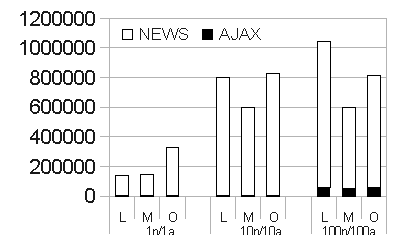
\includegraphics[width=2.5in]{LowConcurrencyThroughput}
\caption{Low Concurrency Throughput}
\label{fig:low_concurrency_throughput}
\end{figure}


\begin{figure}[!t]
\centering 
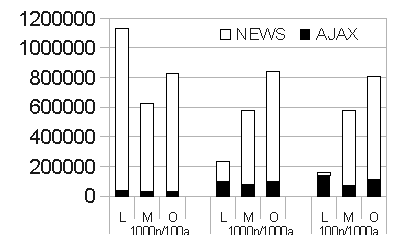
\includegraphics[width=2.5in]{MediumConcurrencyThroughput}
\caption{Medium Concurrency Throughput}
\label{fig:medium_concurrency_throughput}
\end{figure}

\begin{figure}[!t]
\centering 
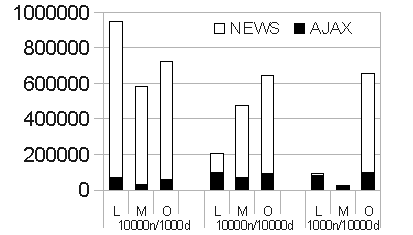
\includegraphics[width=2.5in]{HighConcurrencyThroughput}
\caption{High Concurrency Throughput}
\label{fig:high_concurrency_throughput}
\end{figure}
  


\section{Related Work}
OfficeFloor and its Job Based Architecture is to the best of my knowledge the
first time that the patterns of pipeline, continuations and inversion of control
have been used together along with the abstraction of a thread as a transitive
dependency to achieve a concurrency model that focuses on performance bottleneck
isolation.

Minimising the cost of bottlenecks is one means to improve server performance.
The SEDA Architecture~\cite{seda} reduced the level of service and subsequently
the cost of bottlenecks at higher loads.  Monadic threads~\cite{monadic-thread}
drive the operating system to provide asynchronous resources to avoid blocking
and starvation.  Comparison work identified that servers with smaller footprints
provide more memory for caching and subsequently better
performance~\cite{low-server-footprint}.  While minimising the cost of
performance bottlenecks is important to server performance, findings of this
paper also identify that isolation of performance bottlenecks is important to
overall server performance.

Various abstractions of concurrency have been developed that focus on the task
type.  JAWS provides flexible concurrency components~\cite{jaws}.  Aspen
combines tasks into modules~\cite{aspen}.  Saburo abstracts the concurrency
model via annotations on the tasks~\cite{saburo}.  Hop enables the developer to
provide code to dynamic decide the concurrency model for tasks at
runtime~\cite{hop}.  I however propose the abstraction of the concurrency model
should be based on the thread being a transitive dependency of the task.

Frameworks/libraries have utilised dependencies in their models.  Spring
implements dependency injection~\cite{ioc} however it relies on the Servlet
thread-per-request concurrency model.  Capriccio utilises resource-aware
scheduling of operating system level resources and only suggests scheduling of
application level resources via an API~\cite{capriccio}.  Dependency capsules
focus on isolation for better availability however they do incur thread context
switching overheads~\cite{dependency-capsules} avoided by the Job Based
Architecture.  Flux~\cite{flux} provides extrinsic dependency management
information through task inputs and outputs but focuses on using the information
for task sequencing to avoiding deadlocks rather than bottleneck isolation.

Actors do provide the mechanism to isolate bottlenecks however their decoupling
of message from sender~\cite{actors}, while scalable across distributed nodes,
is not gaining local efficiencies by roles (actors) working across
organisational (iOrg) boundaries for the \textit{smaller} tasks.


\section{Conclusion and Future Work}
Isolation of performance bottlenecks has shown to provide more consistent
performance across differing load profiles by both avoiding creating a
significant number of threads and avoiding thread starvation than
thread-per-request Web Servers.  Furthermore, in many load profiles isolating
the bottleneck provides improved throughput performance.

Future work will look at whether the more consistent throughput performance will
provide improvements in servicing load profiles of real world traffic.
Further comparisons against other web server architectures will be undertaken,
such as event based-architectures to compare developer customisations of
application concurrency against OfficeFloor's transitive thread dependency
concurrency model.  Also, expanding to other Internet services other than web
servers is another area for future work.

Though not discussed in this paper OfficeFloor implements process
continuations~\cite{process-continuation} to provide parallel processing.  I
expect with further research this will prove useful to address performance
bottleneck problems of interacting with multiple downstream systems, such as the
reverse 10K problem~\cite{reverse-ten-k-problem}.







% conference papers do not normally have an appendix


% use section* for acknowledgement
\section*{Acknowledgment} I thank my wife Melanie for her patience and support
in my exploration of the Job Based Architecture through developing OfficeFloor. 
I also thank my friend Matthew Brown for being a sounding board to many of my
ideas.



% An example of a floating figure using the graphicx package.
% Note that \label must occur AFTER (or within) \caption.
% For figures, \caption should occur after the \includegraphics.
% Note that IEEEtran v1.7 and later has special internal code that
% is designed to preserve the operation of \label within \caption
% even when the captionsoff option is in effect. However, because
% of issues like this, it may be the safest practice to put all your
% \label just after \caption rather than within \caption{}.
%
% Reminder: the "draftcls" or "draftclsnofoot", not "draft", class
% option should be used if it is desired that the figures are to be
% displayed while in draft mode.
%
%\begin{figure}[!t]
%\centering
%\includegraphics[width=2.5in]{myfigure}
% where an .eps filename suffix will be assumed under latex, 
% and a .pdf suffix will be assumed for pdflatex; or what has been declared
% via \DeclareGraphicsExtensions.
%\caption{Simulation Results}
%\label{fig_sim}
%\end{figure}

% Note that IEEE typically puts floats only at the top, even when this
% results in a large percentage of a column being occupied by floats.


% An example of a double column floating figure using two subfigures.
% (The subfig.sty package must be loaded for this to work.)
% The subfigure \label commands are set within each subfloat command, the
% \label for the overall figure must come after \caption.
% \hfil must be used as a separator to get equal spacing.
% The subfigure.sty package works much the same way, except \subfigure is
% used instead of \subfloat.
%
%\begin{figure*}[!t]
%\centerline{\subfloat[Case I]\includegraphics[width=2.5in]{subfigcase1}%
%\label{fig_first_case}}
%\hfil
%\subfloat[Case II]{\includegraphics[width=2.5in]{subfigcase2}%
%\label{fig_second_case}}}
%\caption{Simulation results}
%\label{fig_sim}
%\end{figure*}
%
% Note that often IEEE papers with subfigures do not employ subfigure
% captions (using the optional argument to \subfloat), but instead will
% reference/describe all of them (a), (b), etc., within the main caption.


% An example of a floating table. Note that, for IEEE style tables, the 
% \caption command should come BEFORE the table. Table text will default to
% \footnotesize as IEEE normally uses this smaller font for tables.
% The \label must come after \caption as always.
%
%\begin{table}[!t]
%% increase table row spacing, adjust to taste
%\renewcommand{\arraystretch}{1.3}
% if using array.sty, it might be a good idea to tweak the value of
% \extrarowheight as needed to properly center the text within the cells
%\caption{An Example of a Table}
%\label{table_example}
%\centering
%% Some packages, such as MDW tools, offer better commands for making tables
%% than the plain LaTeX2e tabular which is used here.
%\begin{tabular}{|c||c|}
%\hline
%One & Two\\
%\hline
%Three & Four\\
%\hline
%\end{tabular}
%\end{table}


% Note that IEEE does not put floats in the very first column - or typically
% anywhere on the first page for that matter. Also, in-text middle ("here")
% positioning is not used. Most IEEE journals/conferences use top floats
% exclusively. Note that, LaTeX2e, unlike IEEE journals/conferences, places
% footnotes above bottom floats. This can be corrected via the \fnbelowfloat
% command of the stfloats package.




% trigger a \newpage just before the given reference
% number - used to balance the columns on the last page
% adjust value as needed - may need to be readjusted if
% the document is modified later
%\IEEEtriggeratref{8}
% The "triggered" command can be changed if desired:
%\IEEEtriggercmd{\enlargethispage{-5in}}

% references section

% can use a bibliography generated by BibTeX as a .bbl file
% BibTeX documentation can be easily obtained at:
% http://www.ctan.org/tex-archive/biblio/bibtex/contrib/doc/
% The IEEEtran BibTeX style support page is at:
% http://www.michaelshell.org/tex/ieeetran/bibtex/
\bibliographystyle{ieee/IEEEtran}
% argument is your BibTeX string definitions and bibliography database(s)
\bibliography{jba}


% that's all folks
\end{document}


